\chapter{Architecture} \label{cpt:architecture}

\section{Class structure}
The project was separated into several classes. The given framework simple calls
methods which are defined in the package \texttt{at.jku.amp.lepatriinu}.

% \begin{itemize}
%   \ttfamily
%   \item at.jku.amp.lepatriinu.Analyzer
%   \item at.jku.amp.lepatriinu.BeatDetector
%   \begin{itemize}
%     \item at.jku.amp.lepatriinu.AutoCorrelationBeatDetector
%   \end{itemize}
%   \item at.jku.amp.lepatriinu.OnsetDetector
%   \begin{itemize}
%     \item at.jku.amp.lepatriinu.GroundTruthPicker 
%     \item at.jku.amp.lepatriinu.HighFrequencyOnsetDetector
%     \item at.jku.amp.lepatriinu.SimpleOnsetDetector
%     \item at.jku.amp.lepatriinu.SpectralFluxOnsetDetector
%   \end{itemize}
%   \item at.jku.amp.lepatriinu.TempoExtractor
%   \begin{itemize}
%     \item at.jku.amp.lepatriinu.InterOnsetTempoExtractor
%   \end{itemize} 
% \end{itemize}

\begin{figure}[htp]
  \centering
  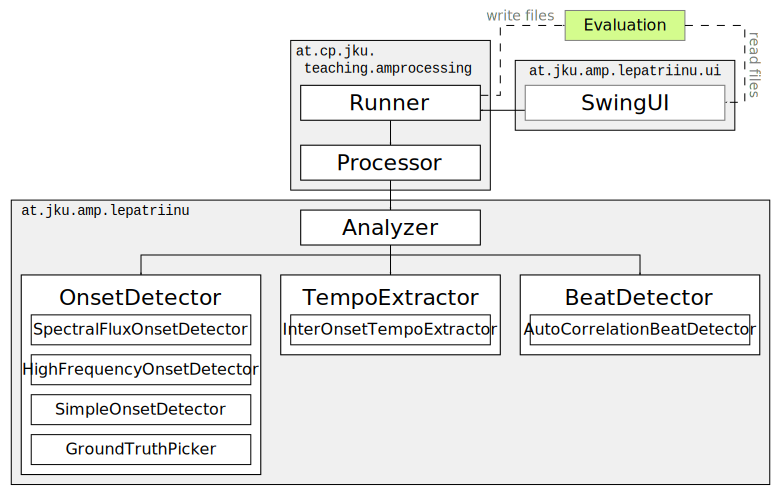
\includegraphics[width=\textwidth]{chapter/ClassDiagram}
  \label{fig:classdiagram}
  \caption{Class diagram}
\end{figure}